\chapter{Simulated Quadrant Photodiode}
\label{chapter:simulated_QPD}

\section{Overview}
In this chapter, we begin with a brief discussion of the working 
principle behind a position detection device. We then provide a 
framework for replicating the scattering signal recorded by a 
quadrant photo diode. We show that extending the framework to 
capture information from an arbitrary shaped particle is simple 
in principle but difficult to interpret, we demonstrate as such 
by comparing the expected signal from a trapped sphere, to that 
of a trapped dimer.

\section{Introduction}

Beyond merely simulating the forces experienced by a spherical 
aggregate we also developed a simulative quadrant photo diode 
to replicate the results from a typical calibration test. This 
builds upon the work from \cite{Rohrbach2002} which applied 
Lorenz-Mie theory to replicate the response signal of a QPD 
being used in back focal-plane interferometry. Rather than be 
constrained to individual spheres we can now consider the 
expected response from any type of spherical aggregate. The
goal of such simulation software would be to simulate the 
expected experimental results from a complex particle whose 
exact shape and size may be difficult to determine. 

In order to simulate a typical experimental set up with a QPD 
installed as a position detection system we need to evaluate 
the total magnitude of the electric field incident on the 
photo-diode surface. While trapping a micro-particle, the 
scattered and incident fields combine together and interfere 
with one another. These fields are collected by a condenser 
lens in the far field limit and are focused onto the QPD 
surface, the total intensity can be evaluated as:
\begin{align}
	I(x,y) = \epsilon_0c\left|
	\begin{bmatrix} 
		E_{i,x}(x,y)+E_{s,x}(x,y) \\ 
		E_{i,y}(x,y)+E_{s,y}(x,y) \\ 
		E_{i,z}(x,y)+E_{s,z}(x,y)
	\end{bmatrix} \right|^2 \times step(\theta_{NA}-\theta(x,y))
\end{align}

The last term is simply a representative step term that defines 
the outer limit by which we evaluate the electric field, this is 
analogous to our condenser lens removing noise from other light 
sources by only accepting light at a specific acceptance angle 
defined by its numerical aperture $NA_c$. Depending on the 
relative size of our particle we can adjust the acceptance angle, 
this has very little effect on the transverse signals, but for 
axial evaluations of a trapped particle the numerical aperture 
should be tuned so that the resultant response curve has negative 
slope in order to allow for axial position detection, the method 
for finding this angle $\theta_\Theta$ is discussed in 
\cite{Friedrich2012}.

The incident beam is simple enough to define given our set up 
parameters, for the sake of simplicity we assume that our beam is a Laguerre-Gaussian 
beam of mode $[0.0, 0.0]$ (which is simply a pure Gaussian beam). 
\textit{Ott} uses a point matching approach to approximate the beam shape 
coefficients of the incident field by fitting it to the far field estimate. 
From the QPD's perspective it is receiving light both from the incident 
and scattered beam simultaneously, as such both fields must be expressed
using outgoing vector spherical harmonics.
\begin{align}
	E_{\rm inc}(r)&=
	E_0\sum^\infty_{n}\sum^n_{m=-n}\left[a_{mn}{\bf M}^{(2)}_{nm}({\bf r})+
	b_{nm}{\bf N}^{(2)}_{nm}({\bf r}) \right] 
	\\
	E_{\rm scat}(r)&=E_0 \sum^\infty_n \sum^n_{m=-n} \left[
	p_{nm}{\bf N}_{nm}^{(2)}({\bf r})+q_{nm}{\bf M}_{nm}^{(2)}({\bf r})
	\right] 
\end{align}

Where the superscript (2) denotes an outgoing spherical harmonic
function. In order to compute the scattering from the target particle \textit{ott} uses the $T$-matrix method, this is not essential 
for a simple sphere but is essential for complex shaped particles 
such as dimers. The scattered and incident fields are then combined 
together in the far field to get $I(x,y)$, the quadrant and overall 
signals are calculated via:
\begin{align}
	Q_i &= \sum_{n,m} I(x_{i,n}, y_{i,m}) \\
	S_{x} &= \frac{(Q_1+Q_2)-(Q_3+Q_4)}{\sum I_0(x,y)} \\
	S_{y} &= \frac{(Q_1+Q_3)-(Q_2+Q_4)}{\sum I_0(x,y)} \\
	S_{z} &= \frac{(Q_1+Q_2+Q_3+Q_4}{\sum I_0(x,y)}
\end{align}

Where the denominator is the total intensity on the QPD while there is 
no particle within the trap. You would expect that $S_x$ and $S_y$ are
near identical for equal particle displacements, however due to the 
polarisation of the beam there will be a slight bias to the signals 
for motion along the direction of the polarisation vector. This is 
generally not an issue if the particle trajectory is sampled for a 
long enough time period. By converting from signal units to length
units (see \eqref{eq:conversion_factor}) the trap shape can be 
discerned from the QPD signals, assuming the fluid properties are
known to a high degree of accuracy.

While translational motion has no knock on effects to the QPD signal, 
rotational changes are double counted by both the incident and total 
field. This results in rotational motion being biased in the QPD signal 
- even when collecting signals from isotropic scatterers. To prevent 
this we need to rotate the total field via the inverse rotation matrix
of the dimer.

To confirm that our method is producing accurate results, we ran a comparison
between our simulative QPD and the results from \cite{Rohrbach2002}. Where a 
$300\ nm$ diameter sphere is scanned across the path of a focused Gaussian beam
($\lambda=1064\ nm$, $NA=1.2$), the sphere has a refractive index of 1.57 and is
suspended in water ($n_{med}=1.33$) and the condenser lens has its numerical aperture
set to 0.5 ($\theta_{max} = 30^\circ$). Scanning across all three primary axis 
produced the following response curve:
\begin{figure}[h!]
	\begin{subfigure}{0.475 \linewidth}
		\subcaption{}
		\includegraphics[width=\linewidth]{QPD_axial_tests.png}
	\end{subfigure}
	\begin{subfigure}{0.475 \linewidth}
		\subcaption{}
		\includegraphics[width=\linewidth]{QPD_lat_tests.png}
	\end{subfigure}
	\caption{Comparison between QPD response signal versus work conducted by 
		Rohrbach, single sphere ($r = 150\ nm$, $n=1.57$) is scanned by a $1064\ nm$ laser and the QPD signal recorded. Solid lines represent the signal 
		produced by QPD using \textit{ott} and points represent the signal 
		response collected from \cite{Rohrbach2002}.}
	\label{fig:Rohrbach}
\end{figure}

The discrepancy between our simulated QPD and the results 
from Rohrbach can be attributed to the fact that the position 
to signal error grows as you move further from trap focus. 
As the particle moves further from the trap focus the error 
in the attributed signal grows substantially \cite{Rohrbach2002}.
In most optical trapping experiments we usually are calibrating 
a strong trap where the mean square displacement falls well within 
the linear regime shown in fig.~\ref{fig:Rohrbach}. In which case 
the error between Rohrbach's model and our own is inconsequential 
for calibration purposes. With this any trajectory can be collected 
from the QPD by displacing and rotating the beam accordingly, 
later in chapters \ref{chapter:langevin_dynamics} and \ref{chapter:simulated_detection} we discuss the limits of 
accuracy that can be achieved using back focal plane interferometry 
to characterise non-spherical targets.

\subsection{Position detection}
\label{sec:position_detection}
In order to accurately capture the dynamics of a trapped particle, a 
position detection system is required. There are 3 possible methods 
of position detection: video-analysis, lateral-effect position sensing, 
and photodiodes. 

Video analysis is ideally suited for multiple traps or situations where 
precision is not the top priority. Whereas lateral-effect and photodiode 
position detection are two examples of back-focal plane interferometry, 
where the interference pattern produced by the target particle is 
extrapolated to determine its position. In order for video analysis to 
match the accuracy of back-focal plane interferometry methods requires 
the camera's frame rate to exceed $1\ kHz$ which can be difficult to 
achieve while maintaining a decent resolution \cite{Gibson2008}. In 
comparison off the shelf back-focal plane detectors can achieve temporal 
resolutions anywhere from $10-100\ kHz$ \cite{BergSoerensen2004}. 

A lateral-effect sensor has a similar output but works using a the 
entire sensor as a single cell analogous to the focal plane of the 
trapping beam. The four corners of the sensor act as anodes connected 
to a base plate cathode, as the beam moves across the surface of the 
detector each anode will experience a different photocurrent depending 
on how close the centre of the interference pattern is to each anode. 
The advantage of a lateral effect detector is that the linear regime 
is much larger than a QPD making it much better for monitoring the 
position of a trapped particle. However, Lateral-effect sensors are 
often limited in their spacial resolution due to high signal-to-noise 
ratios, requiring a high intensity of light on the sensor in order to 
get a clean signal. As a result, most optical force measurements are 
conducted using a QPD as opposed to a lateral-effect sensor, as often 
the displacement is small enough that the signal-displacement curve 
can be considered linear.
\begin{figure}[h!]
	\centering
	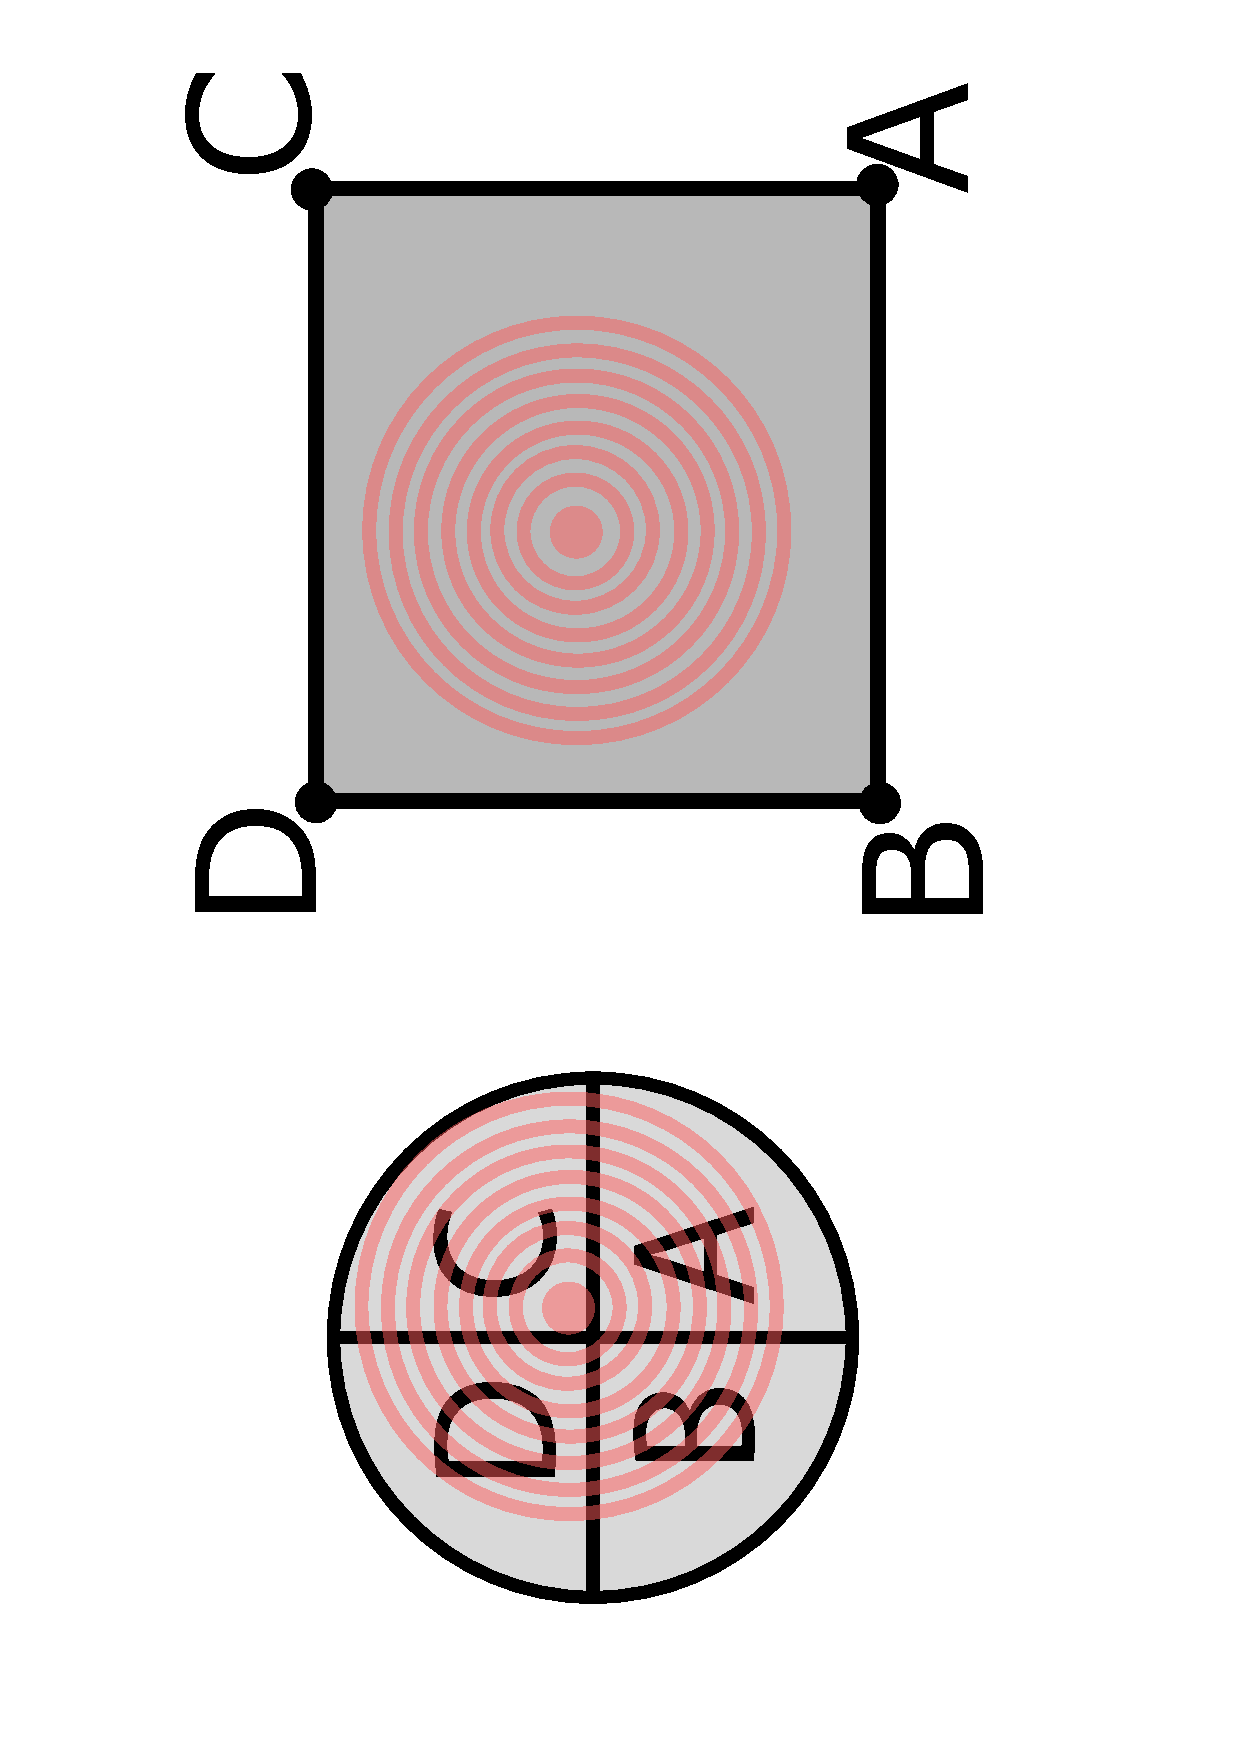
\includegraphics[height=\linewidth, angle=270]{QPD_Lateral_effect.pdf}
	\caption{Comparison between QPD and Lateral effect photodiodes.
		The four quadrants of a QPD (left) experience different photocurrents
		based on the total intensity of light incident on each section 
		(labelled A, B, C, D). 
		Whereas a Lateral effect sensor (right) uses the resistive properties
		of the photodiode surface to vary the create different photocurrents 
		passing through the anodes A, B, C, and D.}
\end{figure}

A quadrant photo diode (QPD) is a frequently used position detection 
system for optical tweezers due to their high sampling rate, high 
degree of precision, and ease of set up. The QPD is constructed of 
four photo diodes assembled in a quadrant formation, when a particle 
is trapped the interference pattern produced is focused onto the QPD, 
with the maximum intensity mapping to the particle's centre of mass. 
By summing the voltages of the horizontal and vertical quadrants together 
the particle's centre of mass is tracked in the $x-y$ plane. Axial 
displacement can be estimated by observing the change in the total 
voltage of the QPD. The outputted signal gives an indication of the 
particle's relative displacement from the beam focus, but in order to 
convert the signal to distance units the trap needs to be calibrated 
(assuming a linear response curve).

\section{Characterisation of asymmetric dimer dynamics via PSD analysis}
As discussed in \ref{sec:simulated_QPD}, one of the methods 
developed to work in conjunction with \cite{Vigilante2020} 
is a simulated quadrant photo diode for as a position 
detection system. While it is possible to extract all of 
the relevant dynamics from a simulation, from an experimental
standpoint characterising those dynamics is dependent on what
experimental techniques are used. Translational motion can be
characterised via a position detection system but angular 
motion is far more difficult to detect, let along characterise. 

The simulative QPD is composed of 4 photodiodes that measure the 
intensity of light incident on their surfaces. Given that the 
condensing lens will have a maximum acceptance angle given by 
its numerical aperture ($\theta_{max} = \sin^{-1}\left(NA_c/n_
{med}\right)$) we define the electric field incident on the QPD 
surface as the elements of the scattered and incident field that 
propagate within that angular range of $\pm \theta_{max}$. Using 
\textit{ott} we can evaluate the total electric field to an 
arbitrary spacial resolution across the surface of the QPD. The 
reported signal is found by taking the difference between pairs 
of quadrant signals (see \ref{sec:simulated_QPD} for further 
detail). This does not provide a one-to-one result however as 
hardware errors (i.e. internal resistance, external light sources, 
and vibrations) would distort the signal. It can be used however to 
show how if the reported power spectra is an accurate representation 
of the true particle dynamics or if the additional degrees of freedom 
have an adverse effect on the scattering. See chapter 2 for a breakdown
of power spectral analysis. 

As a benchmark we start by considering a single sphere within an optical 
trap. A single polystyrene sphere suspended in water ($a=1\mu m$, 
$n_p=1.59$, $n_m=1.33$) was trapped by a focused Gaussian beam ($NA=1.25$) using circularly polarised light. For the sake of time efficiency the trajectory was sampled every 10 time steps, meaning the upper bound on 
the power spectra is $f_{Nyq}=f_{sample}/2=5000\ Hz$. To optimise the 
frequency window we fitted the power spectra using the aliased Lorentzian.
(Eq.~\eqref{eq:aliased_lorentzian}). 
\begin{figure}[h!]
	\centering
	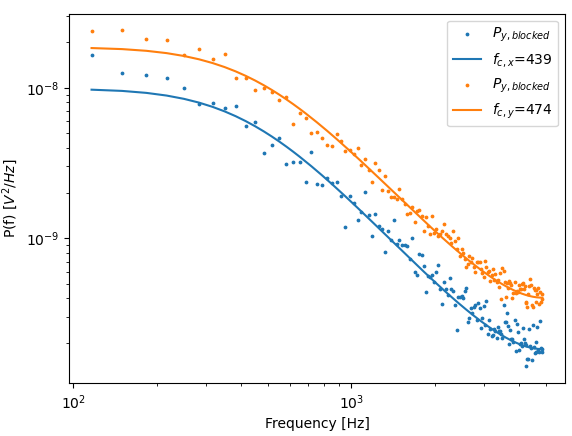
\includegraphics[width=\linewidth]{PSD_sphere.png}
	\caption{Recorded power spectra fitted to eq.~
		\ref{eq:alaised_lorentzian}, scattered points represents 
		the blocked data ($n_b=100$). Corner frequency for the 
		Lorentzian curves are reported in the legend.}
	\label{fig:psd_sphere}
\end{figure} 

As shown in fig.~\ref{fig:psd_sphere}, the two power spectra 
report different corner frequencies which would be indicate 
that the trap is not perfectly circular. We can use both 
\textit{ott} and the trajectory itself to derive an estimation 
of the trap geometry. Additionally, we fitted the 
same Lorentzian to the sphere's positional data, this would be a
situation when the QPD signals are completely uncorrelated with 
one another and there is a constant ratio between the QPD signal 
and the sphere's position. The corner frequencies and corresponding 
trap stiffness are reported below:

\begin{center}
	\captionof{table}{QPD fitting for single sphere}
	\begin{tabular}{ |c|c|c|c|c|c|c| } 
		\hline
		Fitting parameter & \multicolumn{2}{|c|}{\textit{ott} estimates} 
		& \multicolumn{2}{|c|}{QPD fitting} & \multicolumn{2}{|c|}{Trajectory 
			fitting}\\
		\hline
		$f_c\ [Hz]$ & 447 & 450 & \parbox{1cm}{\centering 439} & 474 
		& \parbox{1.25cm}{\centering 523} & 513 \\
		$\sigma(f_c)\ [Hz]$ & --- & --- & 9.30 & 9.65 & 8.67 & 8.61 \\
		$\kappa\ [pN/\mu m]$ & 53.05 & 53.40 & 51.96 & 56.09 & 61.94 & 60.7 \\
		\hline
		Ellipticity &
		\multicolumn{2}{|c|}{8.16 \%} &
		\multicolumn{2}{|c|}{27.17 \%} &
		\multicolumn{2}{|c|}{13.8 \%} \\
		\hline
		
	\end{tabular}
\end{center}

Where $\sigma(f_c)$ is computed from \cite{BergSoerensen2004}, 
where the variance is based upon our choice of frequency 
boundaries ({$f_{min}:f_{max}$} = {$100\ Hz: 5000\ Hz$}). And 
the ellipticity of the beam is given by $e = (1-\kappa_y/
\kappa_x)^{0.5}$ and is a measure of the symmetry of the beam 
wavefront. Its clear from these initial results that the QPD 
is more sensitive to changes along the y-axis than the x-axis 
when compared to the direct \textit{ott} calculations. This is 
somewhat reflected in the trajectory results. Typically, even 
an industrial Gaussian beam will produce an elliptical diffraction 
limit spot when heavily focused; in their tutorial for optimizing 
the PSD analysis, Berg and Sorensen reported a ellipticity of 
around 15 \% after a total calibration time of 80 seconds 
\cite{BergSoerensen2004}.

The reason for the discrepancies between all 3 methods is due 
to what is actually being measured. The \textit{ott} estimates 
are simply looking at the change in the trapping force as you
move along a given axis'. In reality, a particle will be freely
diffusing within the trap focus meaning over a short calibration 
time the QPD is only estimating a weighted average of the trapping
strength. If calibrated over an long enough time frame you would 
expect that the resulting power spectra would exactly mirror the 
\textit{ott} predictions. There is a clear trade off in terms of 
accuracy and computation time as shorter calibration runs are 
computationally more efficient but prone to errors. However, it
should be noted that the estimation made by the QPD is still less
than the results from \cite{BergSoerensen2004}, though this could
be due to a lack of external noise signals.

With this in mind, let us consider a symmetric dimer that is 
optically trapped by the same Gaussian beam. Not only does 
the dimer's equilibrium position change but it is subjected 
to rotational motion due to its unequal moments of inertia. 
This is reflected in the calibration results using the simulated 
QPD, where we see a drastically different estimation between the 
\textit{ott} estimate and the QPD estimate.
\begin{center}
	\captionof{table}{QPD fitting for symmetric dimer}
	\label{tab:dimer}
	\begin{tabular}{ |c|c|c|c|c|c|c| } 
		\hline
		Fitting parameter & \multicolumn{2}{|c|}{\textit{ott} estimate} & 
		\multicolumn{2}{|c|}{QPD fitting} & \multicolumn{2}{|c|}{Trajectory fitting} \\
		\hline
		$f_c\ [Hz]$ & 445 & 409 & \parbox{1cm}{\centering 431} & 424 
		& \parbox{1.25cm}{\centering 274} & 285 \\
		$\sigma(f_c)\ [Hz]$ & --- & --- & 9.22 & 9.16 & 7.82 & 7.91  \\
		$\kappa\ [pN/\mu m]$ & 52.82 & 48.54 & 51.13 & 50.26 & 32.45 & 33.75 \\
		\hline
		Ellipticity &
		\multicolumn{2}{|c|}{28.5 \%} &
		\multicolumn{2}{|c|}{12.7 \%} & 
		\multicolumn{2}{|c|}{13.8 \%} \\
		\hline
	\end{tabular}
\end{center}

Now we see that the \textit{ott} predicts a more elliptical 
trap compared to the QPD model which says the trap is far
more symmetrical while trapping a symmetric dimer. A potential 
reason that \textit{ott} no longer expects a circular trap 
is because that unlike a sphere, the force displacement 
curve is not strictly harmonic. If we consider a dimer that 
is some distance from the beam axis, the sphere closest to 
the trap focus will experience a slightly greater force 
compared to the sphere further from the trap. As such its not
accurate to assume that the external force $F(x) = \kappa x$
instead we must consider that it is a function of both the 
position and orientation simultaneously. 

This coupling of the translational and orientational motion 
has been highlighted previously \cite{Vigilante2020}, but 
there effects have not been demonstrated in the context of
an experimental situation. We can see from the difference in
trajectory and QPD fittings that while our description of the
trap shape is very similar (both methods give similar ellipticity
values) but the magnitude of the trap strength are significantly
different. This is partially explained by the fact that the
QPD is not actually measuring the position of the particle
but instead the intensity distribution of the total field 
incident on the QPD surface. In which case if the dimer is 
rotated slightly the QPD signal will change even if the dimers
centre of diffusion remains stationary. 

\subsection{QPD for angular displacement detection}
The next logical step is to consider whether or not a QPD can at 
all be utilised for detection of rotational motion. This has been
shown for nano-particles that exhibit periodic rotational motion
using by considering the difference in diagonal quadrants 
\cite{Yifat2021}. The only difference between these results is 
the fact that rotation occurs perpendicular to the particle's long 
axis, whereas dimers rotate about their long axis. The benefit of 
detecting rotational motion is that one can begin to build a better understanding about how angular momentum is transferred to a dimer 
which could be extended to more complex particles. This could give 
some understanding to the results of Chapter 4. 

At just a cursory glance it would appear that there is a clear
relationship between the QPD signal and the orientation of the 
dimer. If we look at the QPD signal produced by a dimer as it is 
rotated we can see that it is equally sensitive to rotations in
either the X-Z or Y-Z plane but there is no change in the signal 
when rotated by in the X-Y plane. 
\begin{figure}
	\centering
	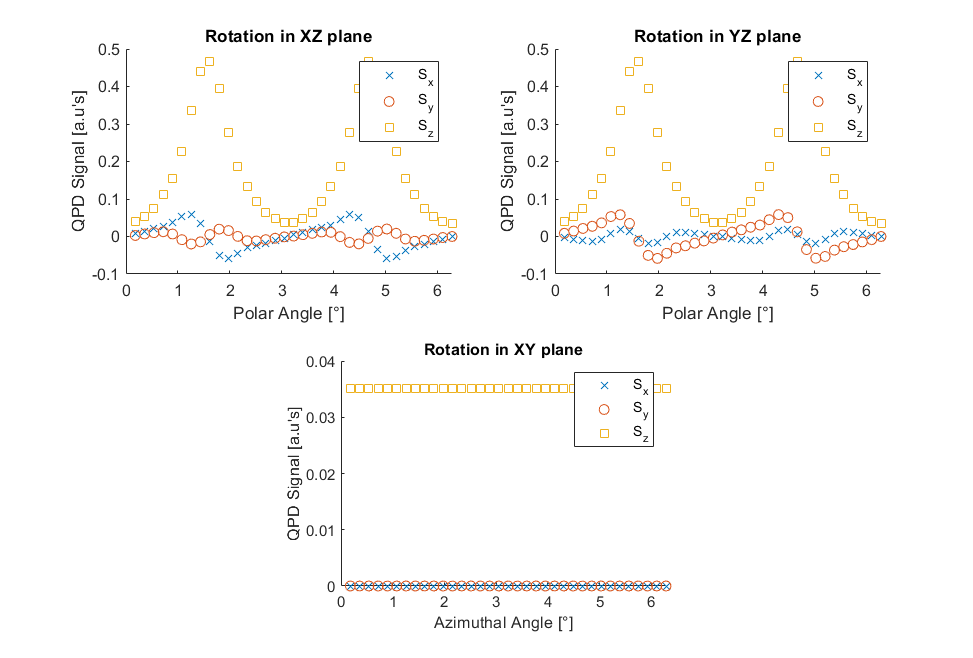
\includegraphics[width=0.9\linewidth]{rotation_figure.png}
	\caption{QPD signals detected by a dimer being rotated while
		centred at the focus of the optical trap. Top right:
		rotation in the X-Z plane. Top left: rotation in the
		Y-Z plane. Bottom: Rotation in the X-Y plane.}
	\label{fig:QPD_rotation}
\end{figure}

However if we compare this to fig.~\ref{fig:rohrbach} we can see 
that the the signal change is dwarfed by the translational motion. 
So while their is a clear relationship between the two trying to
discern between translational and rotational contributions to the
QPD signal is not a simple task. This is significant because it 
means that with regards to the power spectrum fittings in table 
\ref{tab:dimer} there is no way of ensuring that the measured 
trap strengths are accurate. The variance $\sigma(f_c)$ is only 
the variance based upon our fitting parameters and not on the 
actual dynamics of the dimer. In the case where the particle's
shape is not known prior its not possible to determine whether 
any inaccuracies in the power spectra are due to the fit or due
to the particle's motion.

The dependence of $S_x$ and $S_y$ and the dimer's orientation
(defined by the spherical angles $\theta$, $\phi$) is therefore
not clear. To that end, we utilised machine vector regression,
which takes as an input the voltage from the 4 quadrants and 
tries to fit that to the dimer's trajectory. Fitting the QPD
signal to the dimer's position shows promising results, shown in
fig~\ref{fig:QPD_rotation} is a prediction of a symmetric dimer's 
position based on the QPD signal. With the actual displacement 
on the x-axis and the predicted result y-axis, and the dashed 
line represents the y=x line - indicating an ideal prediction. 

Fig~\ref{fig:QPD_rotation} shows that its relatively trivial 
to predict a particle's position based off the QPD signal, even 
in axial direction which has not been done previously. It should 
be noted that these displacements are relative to the trap focus 
and so accurate tracking of the beam movements needs to be taken. 
This result is partially due to the fact that displacement and 
signal units are linearly related by \eqref{eq:conversion_factor}. Interestingly when we run the same protocol for different sized 
dimer's there seems to be a cut off point when the fit begins to 
fail. Plotting the $R^2$ for each fit vs its size ratio shows 
that beyond a size ratio of 5 the machine learning begins to fall 
off significantly. 

This is surprising because we would expect that as the second 
sphere shrinks the dynamics should more closely approximate that 
of a single sphere. This should be reflected in the total field
incident on the QPD and therefore the machine learning program 
should be able to easily detect the dimer's translational motion.
We can therefore only conclude that the dimer's rotational motion
is contributing to the scattering to the scattered field, even if
it is miniscule the contribution is enough to throw off a 
position detection system. Detection of rotational motion was 
attempted using machine learning, the model was trained on the 
same trajectory mentioned in \ref{sec:off-axis}, where the dimer 
is trapped in an off-axis orientation, from a top down perspective
it should be easy enough to note that the dimer is not vertically 
trapped even if the exact angle is difficult to determine. 

Overall, the reliance on machine learning to perform vector 
regression on the collected scattered field is not a viable 
method for detecting let along characterising the angular 
displacement of an isotropic scatterer. While there is a 
clear correlation in the scattered signal and angular 
displacement the translational motion makes up the majority 
of the expected signal detected by the QPD. As of now, there
is no optical arrangement that would allow rotational motion 
while restricting translational motion. 

